\subsection{Spectral analysis and compression of quaternion graph signal}

For this example, let us move away from the UK graph and consider a problem with a much larger network. We select 1000 of the United States (US) counties and, . Using their geographic coordinates, a simple nearest-neighbors approach may be used to infer the underlying undirected graph, as depicted in Figure \ref{fig:us_graph}. In order to define a quaternion-valued signal over this graph using real-world data, we propose taking four variables from the same context or problem and assigning each to a quaternion component. The \textit{ad hoc} constraint of having the variables picked from similar areas is an attempt to make the quaternion graph signal meaningful, so each sample makes sense as a whole.

\begin{figure}
\centering
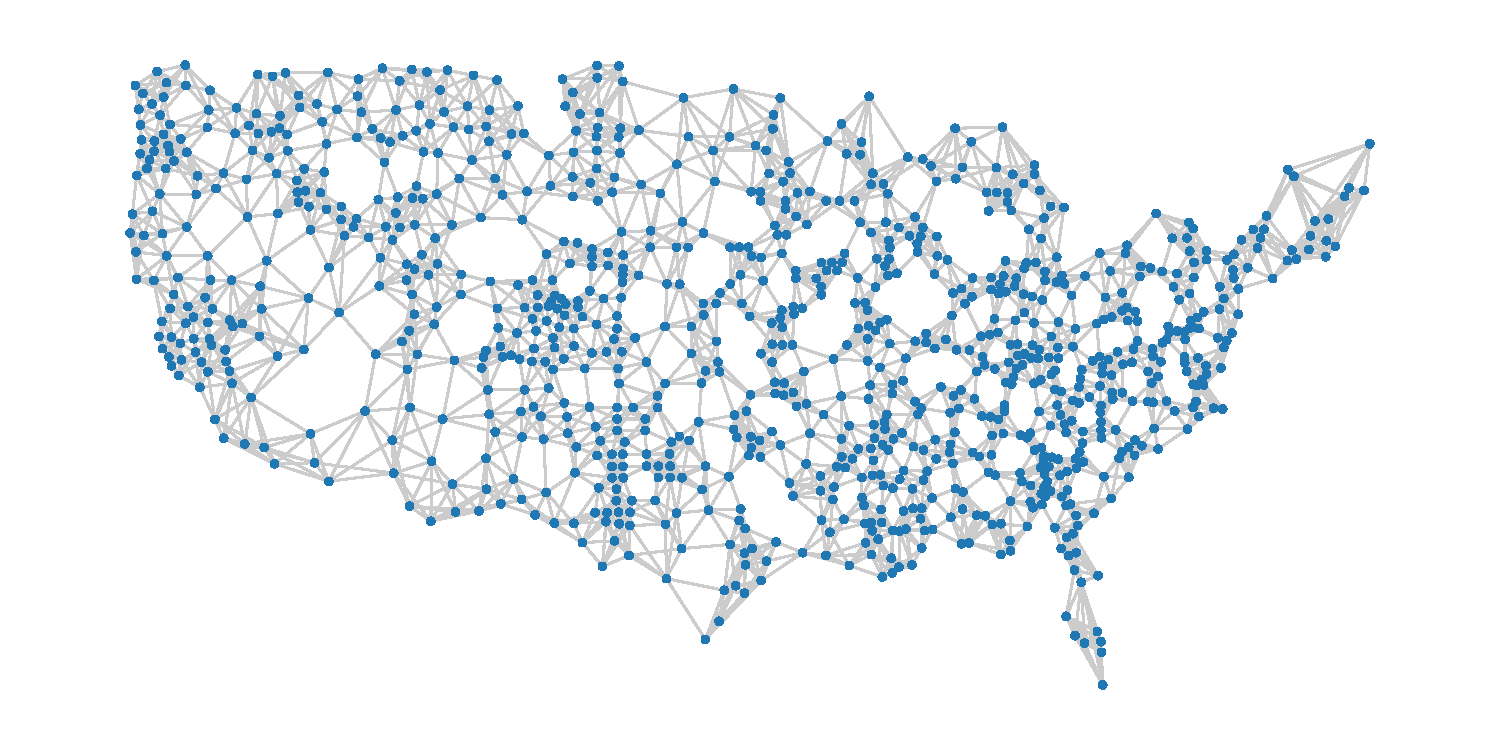
\includegraphics[width=0.8\linewidth]{thesis/Figures/us_graph.pdf}
\caption{Nearest-neighbors graph of a few of the United States counties.}
\label{fig:us_graph}
\end{figure}

For this example, the data was taken from OpenIntro, a non-profit organization focused on spreading high-quality open-source publications. The full dataset\footnote{Avaiable at \url{https://www.openintro.org/data/?data=county_complete}, accessed in October 2022.} comprises 188 variables for each of the 3142 US counties, but only the four sociodemographic indicators were used:
\begin{itemize}[noitemsep]
    \item \textbf{bachelors\_2017}: percent of population that earned a bachelor's degree in 2017.
    \item \textbf{median\_household\_income\_2017}: median household income as of 2017.
    \item \textbf{unemployment\_rate\_2017}: unemployment rate in 2017.
    \item \textbf{uninsured\_2017}: percent of population who were uninsured in 2017.
\end{itemize}

All variables relate to the financial health of american population. Not surprisingly, the Pearson correlation varies from 15\% to 63\% between the group, as shown in Table \ref{tab:02}.
\begin{table}[!h]
\center
\captionof{table}{Correlation between variables used to define the graph signal.}
\label{tab:02}
\begin{tabular*}{\textwidth}{ccc}
\toprule
& & \textbf{Correlation}\\
\midrule
\textbf{bachelors\_2017} & \textbf{median\_household\_income\_2017} & $0.63$ \\
\textbf{bachelors\_2017} & \textbf{unemployment\_rate\_2017} & $-0.35$ \\
\textbf{bachelors\_2017} & \textbf{uninsured\_2017} & $-0.32$ \\
\textbf{median\_household\_income\_2017} & \textbf{unemployment\_rate\_2017} & $-0.38$ \\
\textbf{median\_household\_income\_2017} & \textbf{uninsured\_2017} & $-0.34$ \\
\textbf{unemployment\_rate\_2017} & \textbf{uninsured\_2017} & $0.18$ \\
\bottomrule
\end{tabular*}
\end{table}

Figure \ref{fig:us_signal} displays each quaternion component as a real-valued graph signal. From the plot (a) to (d), the signals contain the features, respectively: \textbf{bachelors\_2017}, \textbf{median\_household\_income\_2017}, \textbf{unemployment\_rate\_2017} and \textbf{uninsured\_2017}.

\begin{figure}
	\centering
	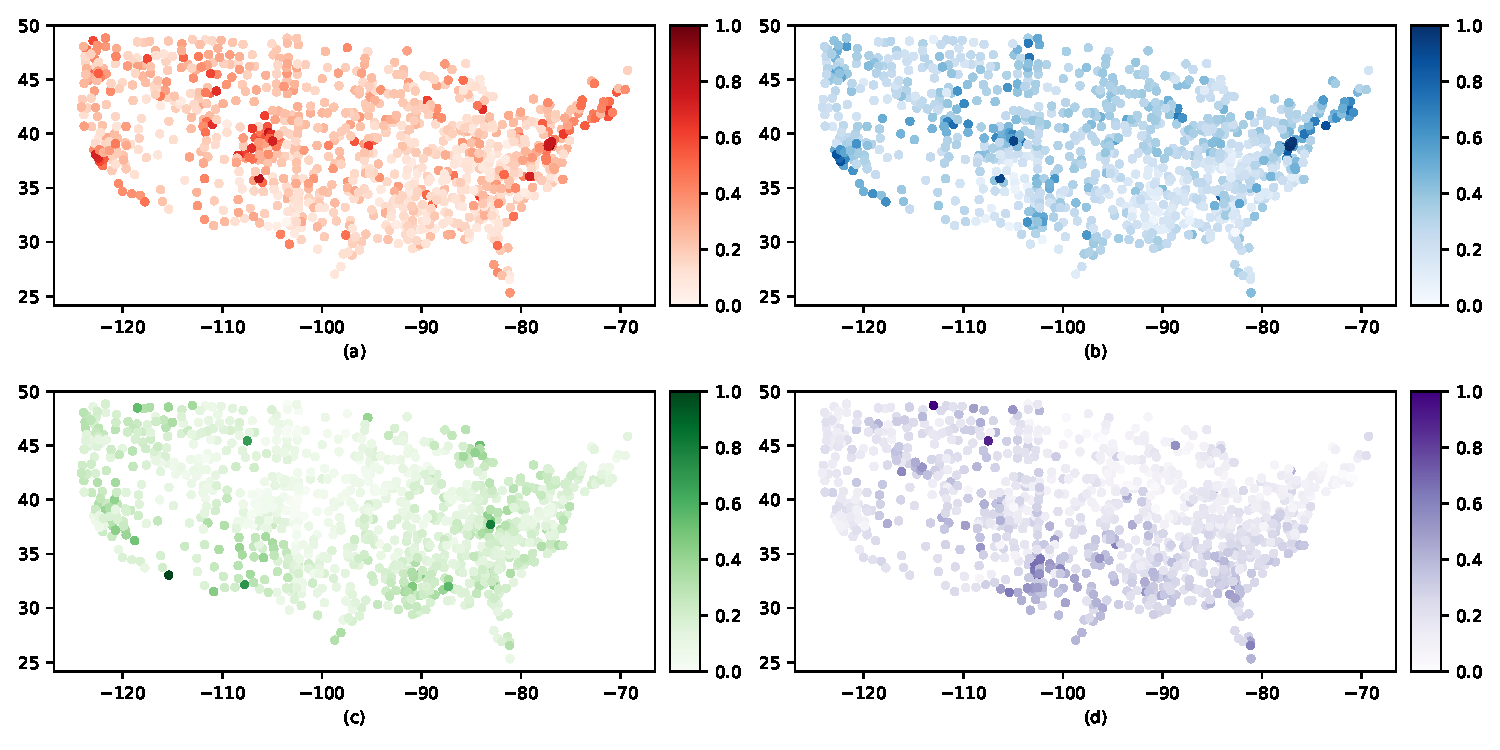
\includegraphics[width=0.95\linewidth]{thesis/Figures/us_signal.pdf}
	\caption{Sociodemographic quaternion-valued graph signal, split into its Hamiltonian components: (a) real part, (b) $\qi$, (c) $\qj$ and (d) $\qk$.}
	\label{fig:us_signal}
\end{figure}

\begin{figure}
	\centering
	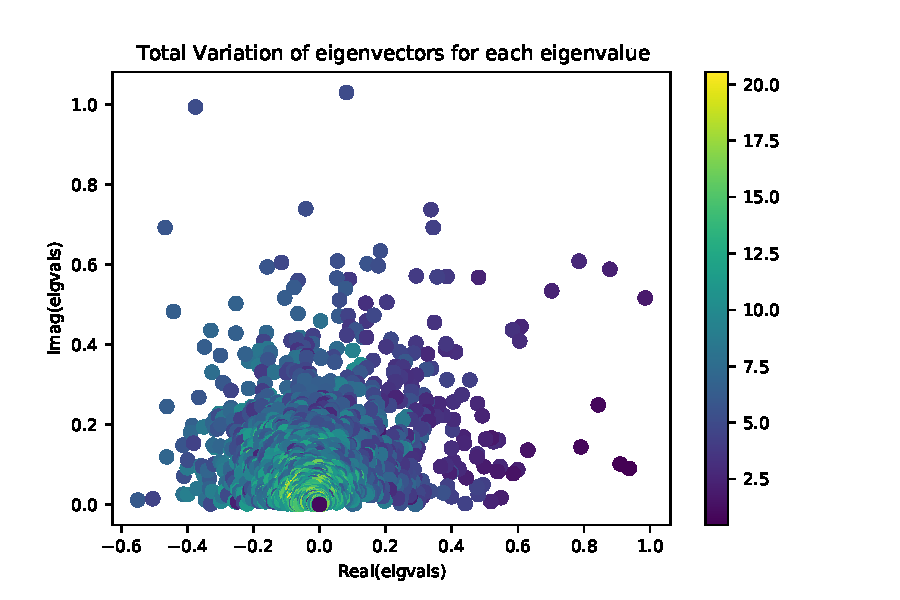
\includegraphics[width=0.7\linewidth]{thesis/Figures/us_counties_qgsp_tv1.pdf}
	\caption{.}
	\label{fig:us_counties_qgsp_tv1}
\end{figure}

\begin{figure}
	\centering
	
\includegraphics[width=0.7\linewidth]{thesis/Figures/us_counties_qgsp_spectrumsig.pdf}
	\caption{.}
	\label{fig:us_counties_qgsp_spectrumsig}
\end{figure}